\chapter{Preventivo}
Di seguito viene riportato il preventivo per il progetto MegAlexa; esso si divide,per ogni periodo,in:
\begin{itemize}
	\item \textbf{Prospetto orario:} presenta la distribuzione oraria e la suddivisione nei ruoli per ogni membro del gruppo ZeroSeven
	\item \textbf{Prospetto economico:}presenta le ore di impegno calcolate per i ruoli coinvolti ed il rispettivo costo 
\end{itemize}
La suddivisione oraria viene svolta avendo come riferimento le seguenti regole:
\begin{itemize}
	\item Ogni membro del gruppo deve coprire ogni ruolo almeno una volta durante il ciclio di sviluppo del prodotoo;
	\item In tutti i periodi tutti i membri devono lavorare lo stesso numero di ore;
	\item Il totale delle ore dovrà essere equamente distribuito tra i membri;
	\item Non ci devono essere conflitti di interesse in cui un Verificatore debba controllare il proprio lavoro.
\end{itemize}
Le sigle utilizzate per i vari ruoli saranno:
\begin{itemize}
	\item \textbf{Re:} Responsabile di Progetto;
	\item \textbf{Ad:} Amministratore;
	\item \textbf{An:}Analista;
	\item \textbf{Pr:}Progettista;
	\item \textbf{Pg:}Programmatore;
	\item \textbf{Ve:}Verificatore;
\end{itemize}

Per il preventivo si tiene conto che i periodi di Analisi dei requisiti e di Consolidamenti dei requisiti sono considerati di investimento del gruppo e  non a carico dei committente, per cui  le ore rendicontate non saranno conteggiate nelle ore totali da retribuire.
\newpage
\section{Attività di  investimento del gruppo}
\subsection{Analisi requisiti}
\subsubsection{Prospetto orario}
Il prospetto orario per il periodo di Analisi è illustrato nella seguente tabella:

\begin{table}[!ht]
  \begin{center}  	
	\begin{tabular}{c}
		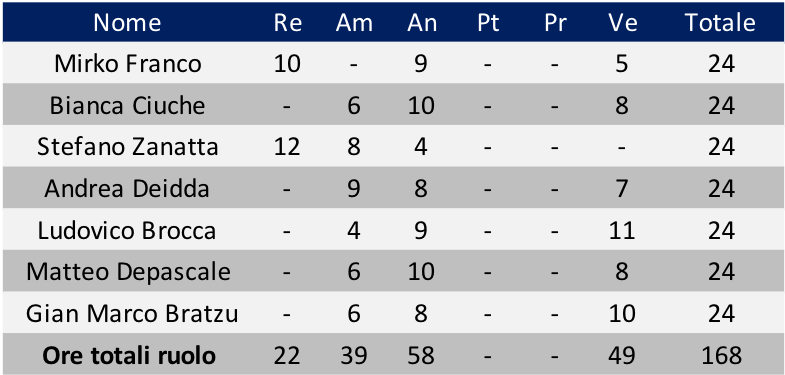
\includegraphics[scale=0.90]{images/tabellaProspettoOrario.png}
		\end{tabular}
		\caption{Prospetto Orario nel periodo di Analisi dei requisiti}
	\end{center}
	\end{table}
Il seguente grafico mostra una rappresentazione visiva della suddivisione oraria dei ruoli:
\begin{figure}[!ht]
	\begin{center}
	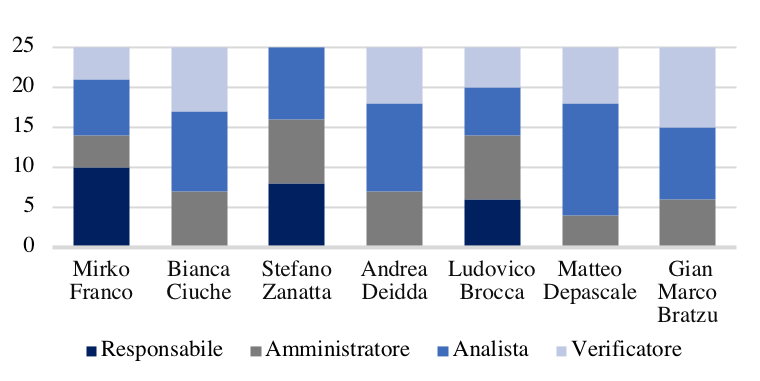
\includegraphics{images/grafoProspettoOrario.png}
	\caption{Grafico prospetto orario nel periodo di Analisi dei requisiti }
	\end{center}
\end{figure}

\newpage
\subsubsection{Prospetto Economico}
Nel periodo di Analisi la distribuzione delle ora tra i differenti ruoli è illustrata nella seguente tabella:

\begin{table}[!ht]
	\begin{center}
	\begin{tabular}{c}
	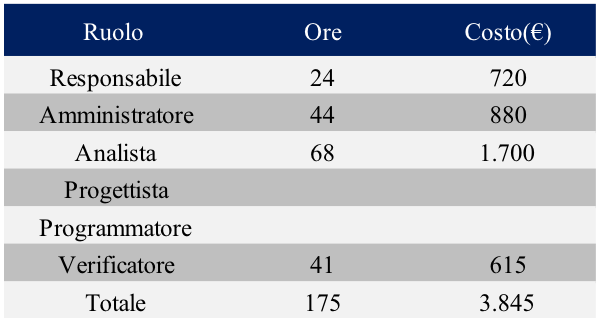
\includegraphics{images/tabellaProspettoEconomico.png}
    \end{tabular}
	\caption{Prospetto Economico nel periodo di Analisi dei requisiti}
	\end{center}
\end{table}

La raffigurazione grafica del peso di ogni ruolo sul costo totale è così rappresentata:

\begin{figure}[!ht]
	\centering
	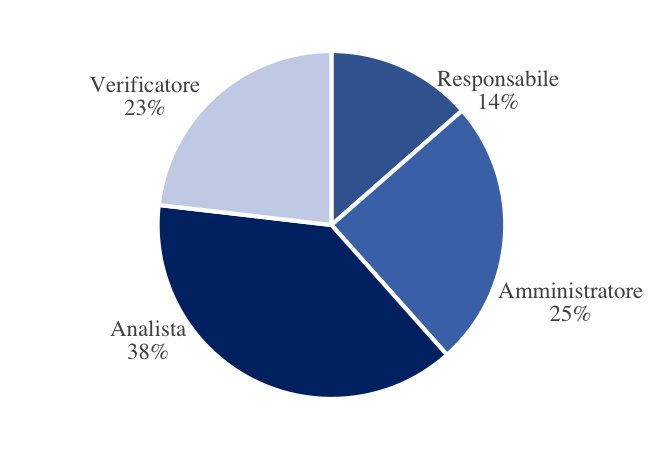
\includegraphics{images/grafoProspettoEconomico.png}
	\caption{Grafico prospetto economico nel periodo di Analisi dei requisiti }
\end{figure}

\newpage
\subsection{Analisi dei requisiti in dettaglio}
\subsubsection{Prospetto Orario}
Nel periodo di Analisi dei requissiti in dettaglio la distribuzione oraria è illustrara nella seguente tabella:
\begin{table}[!ht]
		\begin{center}
	\begin{tabular}{c}
	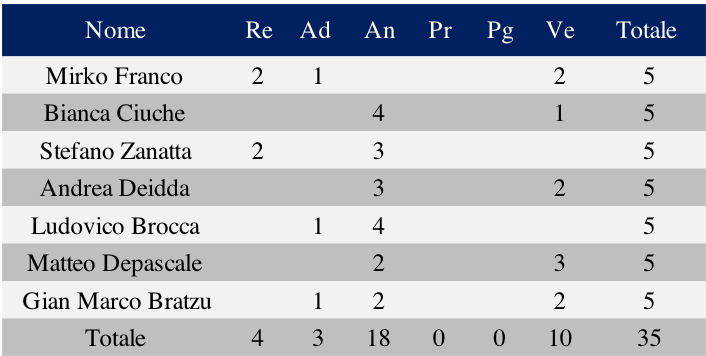
\includegraphics{images/tabellaProspettoOrarioDett.png}
\end{tabular}
	\caption{Prospetto Orario:Analisi dei requisiti in dettaglio}
	\end{center}
\end{table}

Il seguente grafico mostra una rappresentazione visiva della suddivisione oraria:
\begin{figure}[!ht]
		\begin{center}
	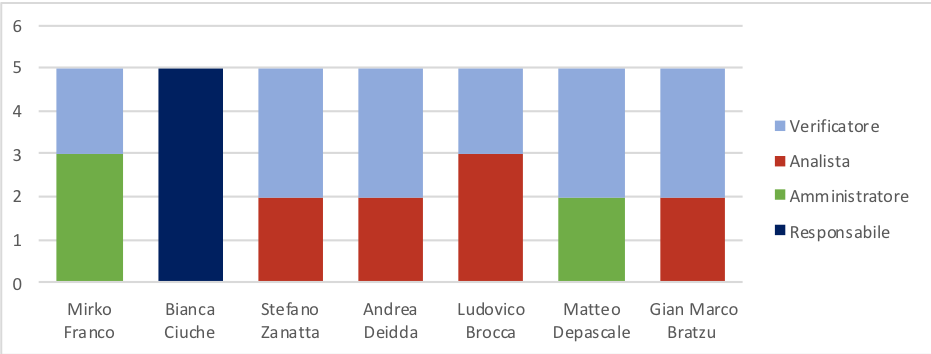
\includegraphics{images/grafoProspettoOrarioDett.png}
	\caption{Grafico prospetto orario nel periodo di Analisi dei requisiti in dettaglio}
	\end{center}
\end{figure}

\newpage
\subsubsection{Prospetto economico}
Nel periodo di Analisi dei requisiti in dettaglio la distribuzione delle ore tra i differenti ruoli è illustrata nella seguente tabella:

\begin{table}[!ht]
	\begin{center}
	\begin{tabular}{c}
	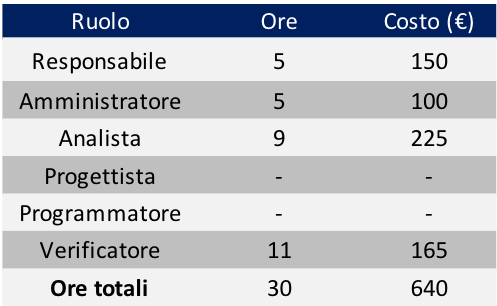
\includegraphics{images/tabellaProspettoEconomicoDett.png}
    \end{tabular}
	\caption{Prospetto Economico nel periodo di Analisi dei requisiti in dettaglio}
	\end{center}
\end{table}

La raffigurazione grafica del peso di ogni ruolo sul costo totale è così rappresentata:
\begin{figure}[!ht]
	\begin{center}
	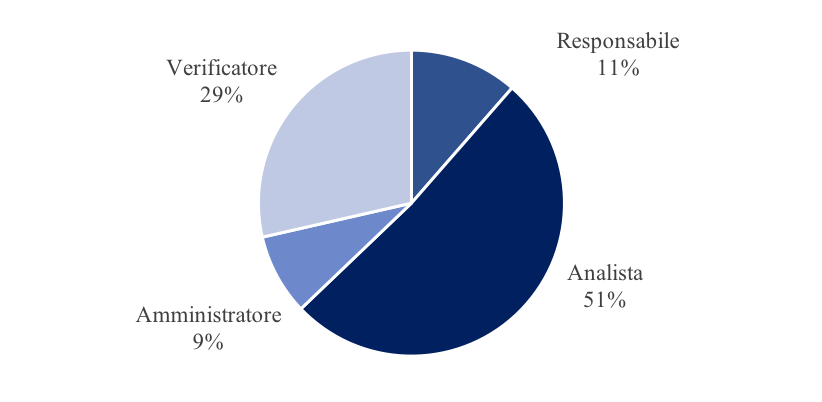
\includegraphics{images/grafoProspettoEconomicoDett.png}
	\caption{Grafico prospetto economico nel periodo di Analisi dei requisiti in dettaglio }
	\end{center}
\end{figure}